\chapter{Design}
\label{cha:design}

Inspired by the success of Transformer architectures on learning sequence modelling tasks in NLP and CV, we propose that we can adapt the same to learn dynamics from network packet data due to the underlying similarity of sequential data. In this chapter, we first present some insights on the data we use for learning, following which, we present the ideas and design choices behind a proposed Transformer architecture which can be used for the same.

\section{Pre-training Dataset}
\label{sec:ns3}
The key requirement for using any deep learning architecture to model and solve a learning problem is the availability good quality training data, which contains enough variation in its  samples in order to capture the underlying distribution effectively. We need enough training data so as the model can learn effectively and not underfit on the training samples. At the same time, we want enough variation in the training data so as to not overfit on a certain subset of features, in order to achieve good generalization benefits from the training process. Given enough data of the right kind, deep learning models are known to exhibit extremely powerful generalizing behaviour\cite{generalizingdnn}.

Acquiring the network packet data to train our proposed NTT model was an initial challenge . A large number of real network traces are sparse (e.g. only 1 hour of data every month) and this is not optimal for training deep learning models. Other kinds of network data while not sparse, is not readily available. Data centres today experience millions of flows per minute across varying levels of granularity and while these can be leveraged to form an ensemble of training data for the specific tasks, the data is usually limited to certain organizations and is not available easily for general use. In order tackle this problem, we use data from network simulations, which allow us to control the ground truth and better understand the performance of the model, while generating data as per our requirement. Latest research has also shown that network simulations and emulations learnt from part of a network and replicated across the varying smaller clusters in the network, can work as almost as well as training on the real network traces, if not the same. Authors in MimicNet\cite{zhangMimicNetFastPerformance2021} have shown the effectiveness and utility of such techniques.

For our task, we use the Network Simulator 3(ns3)\cite{ns3} to generate training and testing data for our NTT. To ensure we capture enough real-world network dynamics, we generate our simulation data from a collection of real world message size distributions, which have been acquired from actual data centres. Given the distribution of these message sizes across multiple workloads, we use ns3 to generate traffic traces from them with varying levels of load.\cite{homa}.

\begin{figure}[h]
  \begin{center}
    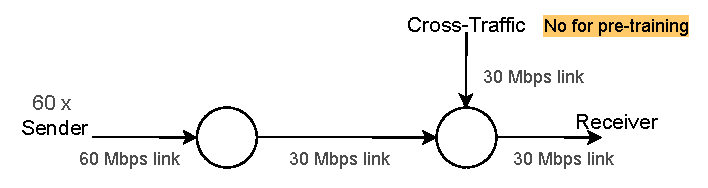
\includegraphics[scale=1.2]{figures/simple_topo.pdf}
    \caption{Initial topology for data generation}
    \label{fig:topo}
  \end{center}
\end{figure}

We begin with a simplified scenario of a single-link network topology which connects two hosts, via two switches as shown in Figure \ref{fig:topo}, where we show the delay Cumulative Density Function (CDF) and the bottleneck queue behaviour. For the pre-training dataset, each of $60$ senders generates $1Mbps$ of messages from the above mentioned distributions. They send messages over a bottleneck link with $30Mbps$ bandwidth and a queue size of $1000$ packets. We run $10$ simulations for $60$ seconds, each with randomized application start times in a $1-50$ second window. This also ensures none of the applications are too short to actually affect the overall dynamics of the network. The randomization of the start times ensures complex interactions between different flows, which lead to significant variation in dynamics of the network. This helps make the data for the pre-training capture a large, generic underlying distribution, which is hugely beneficial for fine-tuning on specific tasks later. This pre-training dataset contains about $1.2$ million packets. There is a possibility of introducing cross-traffic using a second source of disturbance on the second switch, however we turn it off for generating pre-training data, and try to learn general dynamics from a single bottleneck in the topology.

\begin{figure*}[h]
    \centering
    \begin{subfigure}[h]{0.5\textwidth}
        \centering
        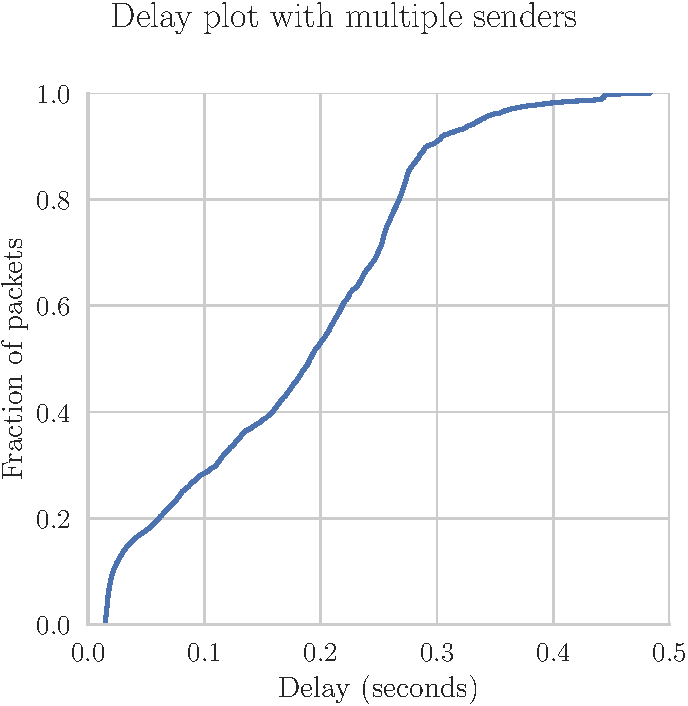
\includegraphics[scale=0.65]{figures/delay.pdf}
        \caption{Delay CDF, single run}
    \end{subfigure}%
    ~ 
    \begin{subfigure}[h]{0.5\textwidth}
        \centering
        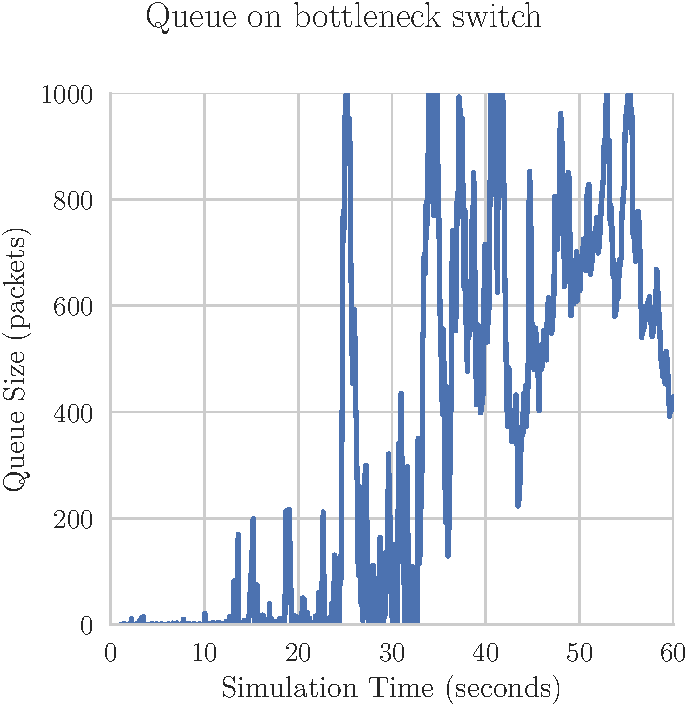
\includegraphics[scale=0.65]{figures/queue_profile_A.pdf}
        \caption{Queue profile on bottleneck queue}
    \end{subfigure}
    \caption{Distribution plots on pre-training data}
    \label{fig:datadist}
\end{figure*}

It is important to ensure that we do not have too much average behaviour in the generated data, else it will prevent the deep learning model from capturing the tail behaviour of the distributions. While in a lot of fields, learning average behaviour with deep learning is more or less enough, this idea fails with network data. In networks, worst-case scenarios can, even if occasionally, lead to significant network outages and data losses. In such an environment, it is crucial to understand the tail behaviour of the traffic distributions across various network applications, in order to truly learn the network characteristics and use the information gained to improve the performance of the network. We ensure that the features required for our training, end to end delay and packet size(we present the choice behind this selection in greater detail in Section \ref{ssec:desfeat}) have enough variation in our training data. We also ensure that the state of the queue on our bottleneck varies throughout the simulation, \ie it is neither always full and nor always empty, which introduces much more variation in the underlying dynamics of the training data. We refer to these distributions in Figure \ref{fig:datadist}.


\section{Network Traffic Transformer (NTT)}
\label{sec:ntt}

We present our proof of concept Network Traffic Transformer(NTT) as a first Transformer model which is trained to learn sequence structure in network packet data and capture the underlying dynamics of the same, and generalize to new tasks based on the transfer learning principles from deep learning . However, learning the structure from network packet data can be extremely challenging. We face several major problems which need to be addressed.

\begin{enumerate}
\item \emph{Complexity of Data:} Network packet data is much more complex as compared to data from images(pixels) or from sentences(words). Packet data comes with several layers of hierarchy in terms of headers, protocol stack etc. We need to devise an effective way to choose features for learning, which captures all of the required information. At the same time, we need to ensure that we don't have redundancy in choosing the features,\ eg some fields across protocols and headers may present the same information in multiple ways. Choosing the features from packets which are the best learning becomes an incredibly hard task.

\item \emph{Time-Series Data:} Neither data in CV nor NLP follows a time series structure, but in network packet data it does, which poses a big challenge. The fate of a packet in the the data depends often on a packet much further in the past, which leads to the need to learn from extremely long sequences of data. As discussed, Transformers scale quadratically with in increasing sequence size, hence learning from long sequences is a challenge. At the same time, the fate of a packet may be affected much more by the more recent packets, which leads to the challenge of effectively learning from both short term and long term dynamics.

\item \emph{Training tasks:} The structure of data in NLP and CV is well understood by humans and it makes it easier to design pre-training and fine-tuning training objectives for these problems. Network packet data is extremely abstract and it significantly harder for us to parse this information and understand it. This makes developing such training objectives on network packet data a bigger challenge. We need to effectively design these in order that the sequence structure can be learnt to the best extent and in the most efficient manner possible.

\end{enumerate}

\begin{figure}[h]
  \begin{center}
    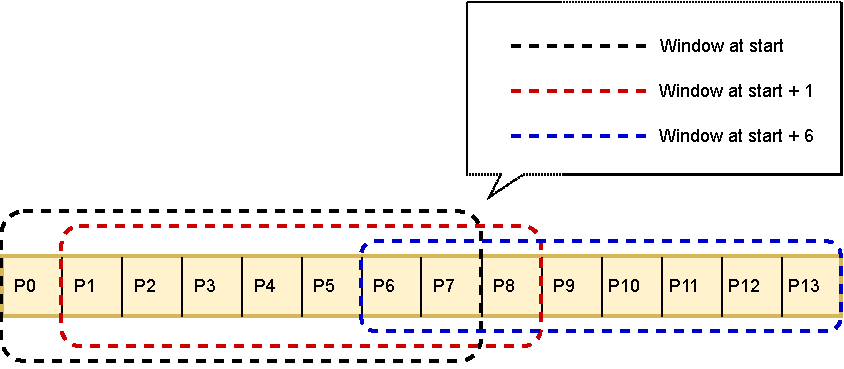
\includegraphics[scale=1]{figures/slidingwindow.pdf}
    \caption{Sliding window for sequence selection. Here P0, P1 etc. represent the features at the packet level used as input to the NTT.}
    \label{fig:sliding}
  \end{center}
\end{figure}


\subsection{Sequence definition}
\label{ssec:desseq}
An initial challenge which came up in our sequence modelling problem was choosing an appropriate sequence definition for our training and evaluation samples. In using Transformers for NLP, the concept of sequence is well defined in terms of either sentences or paragraphs, which come from the structure of most languages itself\footnote{We talk about structure in Indo-European languages here which is not universally true for all language families.} In using Transformers for CV, concept of sequence was artificially constructed using the concept of splitting the image into fixed size patches, which has been covered in detail in Section \ref{ssec:bgvit}. In our case, we have as pre-training data, a time-series dataset, in increasing order of timestamp from the first packet in the network trace.

As our network packet data sequence does not have natural delimiters\footnote{No equivalent of punctuation marks like ``." in NLP.}, we introduce a concept of a sliding window over our packets, in order to create a fixed sequence length, which will then we provided as input to our NTT. We choose a \emph{one-step} sliding window of $1024$ packets,, which roughly matches the size of the queue on the bottleneck switch, over our entire network trace, and each of these windows becomes a single sequence for us. At every step, we shift the sliding window forward by a single step and we illustrate this in Figure \ref{fig:sliding}. We expect that this will capture network behaviour when the queue is full and we hypothesise such a condition to be important for learning the dynamics. The concept of sliding windows has also been successfully used in cases on NLP data, which doesn't have the necessary delimiters in the data itself\cite{beltagyLongformerLongDocumentTransformer2020}, which makes such a design choice a natural starting point in our case. Our sliding window becomes a sequence of elements, which each individual element containing a certain number of features which are required for learning on our training objective.

Our pre-training data contains traces from multiple runs of simulation, in order to increase the richness of our pre-training data and enable us to learn variation in dynamics and generalise to a wide variety of tasks. These simulations represent network measurements taken at different points of time and it is important that our sliding windows always contain elements from the same run of simulation. Since data from different simulation represents independent measurements, we ensure that we construct our sliding windows independently over each run of the simulation data, and then use the data from the combination of these sliding windows as our training samples.

\subsection{Feature selection for the NTT}
\label{ssec:desfeat}

Packets carry a lot of information that could be used as model features, \eg all header fields, payload size etc. Today, we typically use networking domain knowledge to manually extract and aggregate features, then feed them into off-the-shelf standard ML architectures. This is done repeatedly for every task required, we always choose features which will be the best choice for learning our task objective and then, train a new ML model from scratch for every application.
We argue this is sub-optimal for two reasons:
\begin{itemize}
\item First, we always tailor these features to a specific task and dataset, which limits generalization. This process is redundant and never lets us benefit from previous training experiences and results.
\item Second, since the features are not learned from data, they may end up sub-optimal for the task. Choosing the right features for training an ML model is incredibly hard. The only foolproof method is to perform an exhaustive search over all possible combinations of features, and then choose the best performing set/subset of features. Several methods which do this are GridSearchCV and KFoldCV\cite{scikit-learn} but these methods are extremely slow and resource intensive.
\end{itemize}

We propose to let the model learn useful features from raw data. To learn traffic dynamics from a sequence of packets, we must provide the model with information about the packets as well as their fate in the network. Since we do not want to define a priori how important the individual pieces of information are, we feed them all into a first embedding layer~(see Figure \ref{fig:ntt}). The layer is applied to every packet separately. We also tried variations with using a single embedding for the entire sequence and no embeddings at all, both of which performed extremely poorly. The embedding layer itself is a linear projection layer, which helps increase the representation of the information present in the selected features. Also, as these embeddings are learnable parameters in our NTT, over the training process, the model can learn which is the best representation for our input features, from the point of view of feeding information into the transformer encoder. 

We argue that we need both information about the packet state and the network state to capture the overall network dynamics. In our proof-of-concept NTT, we use minimal packet and network
information and argue that the selected features have enough information to model the network dynamics which is needed for our training objectives.
\begin{itemize}
\item \emph{relative timestamp:} Transformer architectures process items in a sequence in parallel, hence they need some positional information in the input in order to understand the relative order of the elements in the sequence. These positional embeddings can be provided as fixed absolute\cite{vaswaniAttentionAllYou2017} or relative\cite{shaw2018selfattention} or as learned positional embeddings\cite{gehring2017convolutional}. Since our packet data is a time-series sequence, we use the relative timestamp to our first packet as a direct feature for our positional encoding information. The relative timestamp is part of the features passed through the embedding layer, and thus becomes a learnable value for a positional encoding.
\item \emph{packet size:} The packet size is used as a feature as it determines the fate of the packet from the packet state. The size of the packet affects the number of packets which can be accommodated in the queue buffer, \eg larger packets means less packets are present in the queue at the particular point in time. This helps in learning the dynamics of the fate of the packet which is directly affected by the state of other packets.
\item \emph{end-to-end delay:} The end to end delay in our setup includes both the queueing delay of the packet, along with the path delay. This delay reflects the state of the network at any given point of time, as the delay is caused by the complex interaction between packets and also reflects effects of tangible networks conditions such as congestion, packet drops etc.
\end{itemize}

These enable learning embeddings with temporal (evolution of delays over time) and spatial (impact of packet size on the delay) patterns. At this point, the clear hypothesis is that these $3$ features will be needed in some form at least, for the NTT to learn and generalize on the network dynamics. It may also happen that for future versions of the NTT, when fine-tuned on complex topologies, may require additional features to distinguish between differences in the data, in terms of path travelled, subnets they belong to etc. In Chapter \ref{cha:evaluation}, we will investigate need for such further features and discuss the challenge of embedding more such information in Chapter \ref{cha:outlook}. 

\begin{figure}[!hbt]
  \begin{center}
    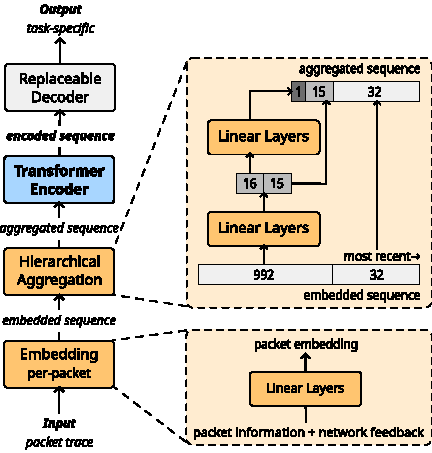
\includegraphics[scale=1.5]{figures/architecture_ntt.pdf}
    \caption{The Network Traffic Transformer (NTT) contains three main stages:  %
        an embedding layer, % for feature extraction,
        an aggregation layer, and
        a transformer encoder.
        It outputs a context-rich encoded sequence that is fed into a task-specific decoder. Credits: Alexander Dietmüller}
    \label{fig:ntt}
  \end{center}
\end{figure}



\subsection{Learning packet aggregation}
\label{ssec:desagg}


As we hope to learn network dynamics, packet sequences must be sufficiently long to capture both the short-term and the long term effects effectively. In Section \ref{ssec:desseq}, we discuss our reasoning behind choosing  $1024$ packets as an appropriate sequence size choice for our initial learning objective. However as the training time of Transformers scales quadratically with the sequence length, we face practical limitations, which we have discussed in Table \ref{bg:table1}. In other fields this is not a a problem, for \eg in NLP, the maximum sequence size in BERT is limited to 512 elements only\cite{devlinBERTPretrainingDeep2019}. Network packet data is extremely fine-grained and depending on the extent of effects we want to capture in our sequence, we may require extremely large sequences of packets, sometimes even in the order of $10000s$ or more.

We address this problem by using multi-timescale aggregation in Figure \ref{fig:ntt}. We aggregate a long packet sequence into a shorter one while letting the model learn to extract relevant historical information from the aggregated sub-sequence.
Coming up with an aggregation scheme which works universally is hard. While coming up with always a fixed aggregation scheme over a constant number of packets is the easiest and probable first choice\footnote{This is similar to the pixel patch aggregation in ViT\cite{dosovitskiyImageWorth16x162021}.}
, we argue that this is suboptimal for two reasons.
\begin{itemize}
\item First, it is not easy to choose such a fixed number, as this might be extremely dependent on the future tasks we want to use our NTT for.
\item Secondly, we hypothesise that due to the nature of structure of packet data, it is more useful to have representation of both aggregated and individual packets.  A fixed aggregation size would mean giving up packet level details completely, which may cause loss in more fine-grained details.\footnote{We do explore the results of fixed aggregation sizes in Chapter \ref{cha:evaluation}.}
\end{itemize}
 
In order to achieve this, we keep the most recent packets without aggregation and the longer traffic is in the past, the more we aggregate, as packet-level details become less relevant to predict the current traffic dynamics. We do this on the argument that most recent information at the packet level is more useful for predict next element's behaviour, whereas individual packets much further in the past matter less and less depending on to which extent in the past they are present.


In our initial NTT experiments, we reduce our initial sequence length of $1024$, using a two layer aggregation scheme, which we aggregate into $48$ elements. The right-hand side of Figure \ref{fig:ntt} shows the aggregation details. We present further details in Table \ref{des:table1}.

\begin{table}[htbp]
\centering
\begin{tabular}{ c   c   c  }
\toprule
Packets in & \# times   & Position in \\
Initial Sequence & aggregated & Final Sequence \\
\midrule
Most recent 32 & None & 16-48 \\
512-992 & Once & 1-16 \\
1-512 & Twice & 1 \\
\bottomrule
\end{tabular}
\caption{Multi-level packet aggregating in the sequence of 1024. The most recent 32 packets are not aggregated, the 480 packets between 512 and 992 are aggregated once, and the packets from 1-512 are aggregated twice. All packets are individually embedded before aggregation.}
\label{des:table1}
\end{table}


Our multi-timescale aggregation can easily be adapted to a larger sizes of past history without sacrificing recent packet details. The initial choice of numbers to map our initial sequence length to our aggregated sequence are slightly arbitrary and do not have a sound theoretical basis yet. We also do not know if matching the packet sequence size to the number of in-flight packets (from the current buffer sizes which give us $1024$ packets) is the best definition of sequence, but it is a logical start, as packets filling into the same buffer, should have closer interactions to an extent. We justify our choice of $48$ as a final sequence length, as given our infrastructure, the Transformer performed reasonably well on these numbers in reasonable training time.\footnote{We will discuss this in further detail in Chapter \ref{cha:evaluation}.} Thus, we show that this aggregation is beneficial for both efficiency and performance, but it remains an open question which levels of aggregation generalize best.\footnote{We will revisit this in the Chapter \ref{cha:outlook}.}


\subsection{Training objectives}
\label{ssec:despatt}

We aim to learn fundamental network dynamics, for which we need a pre-training task which allows us to learn this information from the packet data. As mentioned in Section \ref{ssec:desfeat}, we use end-to-end delay as the feature which represents the fate of the packet in the network. As we argued, almost everything in a network affects packet delays (\eg path length, buffer sizes, etc.). This makes prediction of delays a natural first choice for learning network dynamics, and we need to design a method which allows us to learn this representation. We also know that we can only generalize to a large set of fine-tuning tasks if we have a generic and robust pre-training process. Keeping all this in mind, and given the nature of end-to-end delays as we mention, we feel that capturing the dynamics using this, should be a generic enough task to learn the underlying dynamics.


We take inspiration from masked language models\cite{closemask} in NLP used for training, and argue that masking certain values in a sequence, and reconstructing them, allows for effectively learning the structure in the sequence.

For our initial experiments, we mask the delay of the most recent packet in the sequence to pre-train our NTT.  We used as a fixed mask, \emph{the number $0$}, to replace our actual value, exploiting the fact that the value $0$ never appears in our training data in either the delay or the size values. We can also extend this mask value to more complex data with more features, combining our domain knowledge in networks and shifting possible actual $0$ values by a given constant, using the argument that shifting all values by a constant doesn't change the structure in the data. After the packet is masked, the input sequence is passed through the embedding layer, the transformer encoder, and finally we use a multi-layer perceptron as a decoder to predict the actual delay. As in this pre-training method, we do not have to worry about any of the packets which are aggregated, as those packets are never masked.

During pre-training, the NTT must learn which useful representation from the input features using the embedding layer, how to aggregate them over time using the aggregation layers, and how the aggregated elements influence each other using the transformer encoder layers. Following this, during the fine-tuning, we replace replace the decoder(Figure \ref{fig:ntt}) to adapt NTT to a new environment(\eg a different network) or to new tasks(\eg predicting message completion times).This is efficient as the knowledge accumulated by NTT during pre-training generalizes well to the new task.\footnote{We demonstrate the findings in Chapter \ref{cha:evaluation}.}

Following the initial experiments, we also extend our pre-training process to include the following, newer techniques, with the hypothesis that this makes the pre-training process harder and in turn, more generic. We expect this to be beneficial as it prevents the NTT from overfitting on using all elements in the sequence to always predict a value at the same position, which in our initial design was always at the last position. In order to achieve this, we devise multiple new pre-training methods, where instead of always masking the final delay position, we mask different positions in the sequence, and try to reconstruct the masked value as the pre-training objective. Inspired by the BERT\cite{devlinBERTPretrainingDeep2019} model, we expect to incorporate better bi-directionality in learning sequence structure, given that the position of the masked value to be predicted is not at the end of the sequence, and has neighbouring elements on either side. This in turn, should allow for better learning of sequential structure and dynamics from the packet data.

In our initial NTT design, we only masked the last delay value which was never aggregated and the NTT could directly be trained by reconstruction and comparison against the true value. Now that other delay values will be masked, some of which might be aggregated as per our NTT's design, we propose the modified training objective.

\begin{itemize}
\item \emph{For non-aggregated values:} If the masked delay value in our NTT's input sequence is not aggregated, it corresponds to a single encoded state after passing through Transformer layers. In this event, we train the model by computing the loss against the true delay value, in the given input sequence which was masked out.
\item \emph{For aggregated values:} If we mask a single delay value in our NTT's input sequence, which is then aggregated, there no longer exists a single encoded state, corresponding to this exact value. To handle this, we mask all delay values which are aggregated to the same encoded sequence, in case the individual value is in the aggregated portion of the input sequence. This means that if the delay value is in the twice aggregated subsequence, we mask out $512$ values at a time and if it is in the single aggregated subsequence, we mask out $32$ values at a time. To train the model now, we compute the loss against the mean delay of all actual values, which were masked out in this instance.
\end{itemize}

The \emph{key idea} here is that packets further in the past are hypothesised to have a smaller effect on the value of the current delay, and it should hence be enough to use the average values of delays to train the model to learn the representation from these delays. A-priori, it is not trivial to decide which is the best way to mask variable positions in the input sequence, in order to have better learning of the underlying sequence structure and dynamics. In the scope of our current work, we experiment with several different variable masking strategies, in order to demonstrate that there is not (yet) one true method, which solves this problem universally.\footnote{We present a detailed evaluation on the performance of these NTT pre-training variants in Chapter \ref{cha:evaluation}.}











